\chapter{Модель образования радионуклидов в топливе и теплоносителе ядерного реактора}

\section{Миграция радионуклидов на \ac{aes}}

Как и любое масштабное производство, \ac{aes} выбрасывает в атмосферу и окружающую среду вредные вещества, среди 
которых есть и радиоактивные. При нормальных условиях эксплуатации эти выбросы незначительны, так как современные 
атомные электростанции содержат множество систем очистки сбросов от радионуклидов, однако при нарушении работы 
какой-либо из систем \ac{aes} становится серьезным источником выбросов радионуклидов в атмосферу.

Основные пути распространения радиоактивных нуклидов на \ac{aes} представлены на рисунке \ref{fig_nuclides_spread}.

\begin{figure}[ht]
\centering
	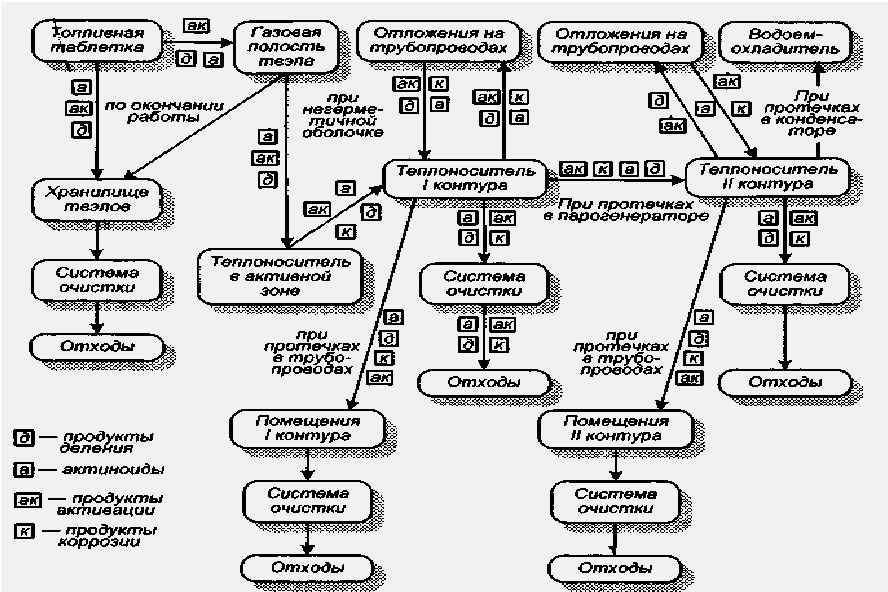
\includegraphics[width=15cm]{nuclides_spread}
    \caption{Основные пути распространения радионуклидов на \ac{aes}.}
    \label{fig_nuclides_spread}
\end{figure}

% Поставить ссылку откуда взята картинка (не обязательно), далее описать барьеры распространения примесей по 
% презентации и лекции "выбросы аэс"
